\section{Introduction}
Among all features of the human body, many can be used to authenticate and authorize people by making use of the incredible natural diversity in human appearances. 
Fingerprints in particular have stood out as one of the most reliable method to identify individuals.
Increased availability and compactness of modern digital capture systems have long surpassed analog methods by speed and deliver results quick enough for every day usage.

With all these benefits some problems such as unsupervised misauthorizations can have catastrophic outcomes.
Malicious intent is often connected to high-value targets like critical infrastructure or border control systems, and successful intrusions can lead to severe consequences.
These authentication systems are operating with a high accuracy with no tolerance for errors, which requires highly specialized and costly hardware.
The expensive components make it difficult to integrate high quality fingerprint scanners into systems that are less critical, but still represent attractive targets for unauthorized access like smartphones and personal computers.

Restricted space and aggressive cost optimization create the need for small capture devices which are easy to use, easy to integrate and cheap to produce. 
The reduction in capture-device quality naturally comes with a reduction of authentication accuracy.
Software enhanced authentication systems can deliver impressive results while not requiring complex capture devices.

\medskip
\subsection{Neural Networks}
Open-Source libraries like Keras offer simple interfaces for complicated software frameworks like Tensorflow and provide ready-to-use machine learning implementations.
A selection of pre-trained convolutional neural networks was used to conduct the following experiments.

\medskip\noindent
Spacial diversity was a category for selecting the algorithms to provide an insight on how complicated a deep-learning network needs to be in order to provide confident decisions on whether a presented fingerprint image is coming from a live person or not.
It is important to note that these networks were meant to be image classifiers detecting the image's contents.
The classifier MobileNet for example, can detect real world objects and animals and is intended for "mobile and embedded vision applications" (cite MobileNets).

\begin{wrapfigure}[13]{r}{7cm}
    \begin{tabular}{| l | r | r |}
    \hline
    Network Name   & Size    & Parameters \\ \hline\hline
    MobileNet      & 16 MB   &   4,253,864 \\ \hline
    NASNetMobile   & 23 MB   &   5,326,716 \\ \hline
    EfficientNetB0 & 29 MB   &   5,330,571 \\ \hline\hline
 
    Xception       & 88 MB   &  22,910,480 \\ \hline
    InceptionV3    & 92 MB   &  23,851,784 \\ \hline
    EfficientNetB5 & 118 MB  &  30,562,527 \\ \hline\hline

    NASNetLarge    & 343 MB  &  88,949,818 \\ \hline
    VGG16          & 528 MB  & 138,357,544 \\ \hline
    VGG19          & 549 MB  & 143,667,240 \\ \hline
\end{tabular}
\caption{Table: Neural Networks}
    \label{tbl:nerual_networks}
\end{wrapfigure}
\noindent
A total of nine different neural networks were categorized by their size and depth into three groups (see Table \ref{tbl:nerual_networks}).
Each network was custom fitted into the task at hand with wrapper-layer encapsulating the original behavior in a non-intrusive way to ensure that the default behavior is sustained.

\smallskip\noindent
The original input layer was discarded and replaced with a generic Input Layer accepting images of size 250x250. All models share the same input layer implementation.
Furthermore, two additional layers were added to the other end of the stack to flatten the neural network's output and to result in a liveliness score between $0$ and $1$.
Sigmoid is used as the activation function.

\noindent
Each neural networks internal behavior is treated like a black box.



\subsection{Dataset}
The provided fingerprint samples were originally used as input material for a conference and competition about fingerprint detection. Various materials were used to present a print resembling a finger.

\begin{wrapfigure}[6]{r}{0.55\textwidth}
    \vspace{-5mm}    
    
    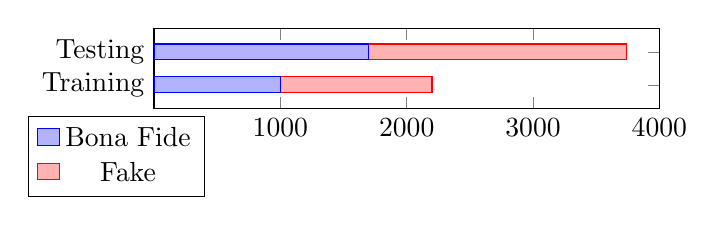
\begin{tikzpicture}
        \begin{axis}[
            xbar stacked, xmin=0, xmax=4000,
            width=8cm,height=2.6cm,
            bar width=2mm,
            xtick={1000,2000,3000,4000},
            xticklabels={1000, 2000, 3000, 4000},
            symbolic y coords={Training,Testing},
            ytick=data,enlarge y limits={abs=3mm},
            legend style={
                at={(-0.25,-0.6)},
                anchor=west,
            }
        ]
            \addplot coordinates { (1000,{Training}) (1700,{Testing})};
            \addplot coordinates { (1200,{Training}) (2040,{Testing})};
            \legend{Bona Fide, Fake}
        \end{axis}
    \end{tikzpicture}

\vspace{-8mm}
\caption{Fingerprint Image Count}
\label{fig:dataset}
\end{wrapfigure}

\noindent
Usually training and validating data are split differently and with relations almost flipped as compared to the dataset provided for LivDet2017 participants.
A train/test split of about 2:1 is often recommended.
Machine learning algorithms get more accurate the more unique data for testing purposes is provided.
Therefore the lack of training data will prove to be an additional challenge.

\begin{wrapfigure}[7]{r}{0.50\textwidth}
    \vspace{-5mm}
    \begin{table}[htb]
    \centering

    \begin{minipage}[r]{0.25\textwidth}
        \centering Training Data (37\%)
        
        \smallskip
        \begin{tabular}{ l r } \hline
            Material    & Share \\ \hline
            Live        & 45\%  \\
            Body Double & 18\%  \\
            Ecoflex     & 18\%  \\
            Wood Glue   & 18\%  \\ \hline
        \end{tabular}
    \end{minipage}
    \hspace{10mm}
    \begin{minipage}[r]{0.25\textwidth}
        \centering Testing Data (63\%)
        
        \smallskip
        \begin{tabular}{ l r } \hline
            Material        & Share \\ \hline
            Live            & 45\%  \\
            Gelatine        & 18\%  \\
            Latex           & 18\%  \\
            Liquid Ecoflex  & 18\%  \\ \hline
        \end{tabular}
    \end{minipage}

    \caption{Material Distribution}
\end{table}

\end{wrapfigure}

\smallskip\noindent
About half (45\%) of both datasets are bona fide fingerprints which leaves the other half comprised of materials emulating human skin.
Different materials were used to train and to validate the neural networks.
Body Double Ecoflex and Wood Glue (each 18\%) were use to train and Gelatine, Latex and Liquid Ecoflex (also each 18\%) are used for validation.
59\% of fingerprint samples are from female subject while 41\% are from males.
Each image was also classified with an age as well.

\begin{wrapfigure}[10]{r}{0.5\textwidth}
    \vspace{-5mm}
    
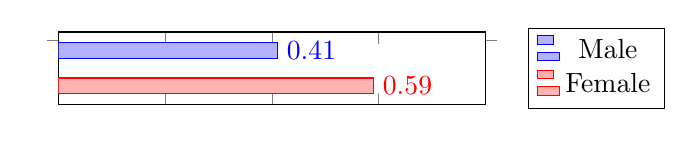
\begin{tikzpicture}
    \begin{axis}[
        xbar, xmin=0, xmax=0.8,
        width=7cm,height=2.5cm,
        bar width=2mm,
        symbolic y coords={F,M},
        ytick=data,enlarge y limits={abs=1mm},
        nodes near coords,
        yticklabels={,},
        xticklabels={,},
        legend style={
            at={(1.1,0.5)},
            anchor=west,
        }
    ]
        \addplot coordinates { (0.41,{M}) };
        \addplot coordinates { (0.59,{F}) };
        \legend{Male, Female}
    \end{axis}
\end{tikzpicture}
\vspace{-5mm}
\caption{Sex Distribution}
    \vspace{2mm}\hrule\vspace{2mm}
    \begin{tikzpicture}
    \begin{axis}[
        height=25mm,
        width=95mm,
        yticklabels={},
        xtick={21, 25, 31.3, 40, 77},
        xticklabels={21, 25, 31.3, 40, 77}]

        \addplot+ [
            boxplot prepared={
                box extend=0.6,
                whisker extend=1,
                lower whisker=19.0, 
                lower quartile=21.0,                
                median=25.0,
                upper quartile=40.0,
                upper whisker=77.0,
                average=31.3
            }
        ] coordinates {};
    \end{axis}
\end{tikzpicture}
\vspace{-2mm}
\caption{Age Distribution}
\label{img:age-dist}

\end{wrapfigure}%

\medskip\noindent
No recognizable variance in prediction accuracy is expected as the diffrence in sex and age do not infer a significant change in fingerprint anatomy or appearance to play a role in this experiment.
With that said, a more mature finger can have noticable damage like scars or common wear from labor and general use.

\begin{wrapfigure}[9]{r}{0.35\textwidth}
    \vspace{-10mm}
    \begin{minipage}[r]{0.15\textwidth}
        \includegraphics[width=\linewidth]{live.bmp}
        \caption{Bona Fide Fingerprint}\label{fig:finger-live}
    \end{minipage}
    \begin{minipage}[r]{0.15\textwidth}
        \includegraphics[trim=32 32 32 32,clip,width=\linewidth]{live.bmp}
        \caption{Sweat Glands}\label{fig:sweat-glands}
    \end{minipage}
\end{wrapfigure}%

\medskip\noindent
All images were captured on a Green Bit DactyScan84C and have a resolution of 500x500 pixel.
The scanner is a standalone high-end device able to capture the fingerprints in high resolution and keeping important details intact.
Bona fide fingerprint images are of such high quality that sweat glands are visible as small white spots on fingerprint ridges in some samples as illustrated in Figure \ref{fig:sweat-glands}.

\medskip\noindent
Training and validation datasets use different materials to fake a fingerprint which adds a level of unpredictablity to the experiment.
Important to note is that none of the used material groups share a distinct property or feature which would make it easier for the trained algorithms to infer the artificiality of unknown materials.

\medskip\noindent
Below is a fingerprint image from each material group.
None of the materials capture sweat glands which my be beneificial to determince whether the presented image is a presentation attack or genuine.

\begin{figure}[!htb]
    \begin{minipage}[r]{0.5\textwidth}
    \begin{minipage}[r]{0.3\textwidth}
        \centering
        \includegraphics[width=\linewidth]{fake-ecoflex.bmp}
        \vspace{-10mm}\caption{Ecoflex}
    \end{minipage}
    \begin{minipage}[r]{0.3\textwidth}
        \centering
        \includegraphics[width=\linewidth]{fake-body-double.bmp}
        \vspace{-10mm}\caption{Body Double}
    \end{minipage}
    \begin{minipage}[r]{0.3\textwidth}
        \centering
        \includegraphics[width=\linewidth]{fake-wood-glue.bmp}
        \vspace{-10mm}\caption{Wood Glue}        
    \end{minipage}
    \caption{Training Dataset}
\end{minipage}
\vrule
\begin{minipage}[r]{0.5\textwidth}
    \begin{minipage}[r]{0.3\textwidth}
        \centering
        \includegraphics[width=\linewidth]{fake-gelatine.bmp}
        \vspace{-10mm}\caption{Gelatine}
    \end{minipage}
    \begin{minipage}[r]{0.3\textwidth}
        \centering
        \includegraphics[width=\linewidth]{fake-latex.bmp}
        \vspace{-10mm}\caption{Latex}
    \end{minipage}
    \begin{minipage}[r]{0.3\textwidth}
        \centering
        \includegraphics[width=\linewidth]{fake-liquid-ecoflex.bmp}
        \vspace{-10mm}\caption{Liquid-Ecoflex}        
    \end{minipage}
    \caption{Validation Dataset}
\end{minipage}
\end{figure}


\newpage


\subsection{Data Acquisition}
\begin{wrapfigure}[13]{r}{10cm}
    \begin{tikzpicture} 
    \begin{umlcomponent}[x=-3,y=0]{Keras} \end{umlcomponent}
    \begin{umlcomponent}[x=3,y=0]{TensorFlow} \end{umlcomponent}

    \umlassemblyconnector[interface=Low Level API]{Keras}{TensorFlow}

    \begin{umlcomponent}[x=2,y=-3]{cnnpad}
        \umlsimpleclass{CnnWrapper}
    \end{umlcomponent}
    
    \umlVHVassemblyconnector[interface=CNN Model Abstractions]{cnnpad}{Keras}


    \umlprovidedinterface[interface=CLI,distance=3cm, with port]{cnnpad}
\end{tikzpicture}
\end{wrapfigure}
Keras is an open-source framework for neural networks and machine learning for the programming language Python.
It offers a simple interface to complex calculations, sophisticated computational resource management and is built on top of TensorFlow (indircite https://keras.io/).

LOOK  HERE Various Python scripts are created for each sequence of the experiment.
Training the networks, saving the trained weights and evaluating the results is done by one pipeline.
Another set of scripts reevaluates best-case trained models and refines the data into human friendly structures.




\subsection{Methodology}
The experiment is split into two parts.
During the first phase the best-case (highest average validation accuracy) for each network needs to be determined.
Due to randomized initial values and subsequent variance in training evolution, the resulting validation accuracy can fluctuate to some degree.
Repetitive training and evaluating will give a set of models for each network which can be serialized and stored.

Models are trained using the provided training dataset over four epochs, which delivered the best balance between validation accuracy and training time.

A total of ten trainings for each network will be used as a pool to pick the best performing model.

\noindent
Trained models are not volatile and can be loaded from disk at any time, so using the best case for each is the fairest approach to make sure every network has the best chances.


\medskip\noindent
Further experiments are conducted in the second phase where the best-case models for each network predicts whether a fingerprint presentation is bona fide or an artificially constructed fingerprint replica.
Unlike neural network training, the predictions of the trained model are static and will not change.
The resulting predictions are used to analyze possible correlations between input data and predicted values.

Just like the original paper about the LiveDet2017 competition, the predictions of each algorithm will be classified by assuming that prediction values of at least 0.50 (cite LiveDet2017) suggest a bona fide fingerprint while all lower values suggest a presentation attack.

